% !TeX root = ../../thesis.tex
\chapter{In-Situ Annealing Effect on Structural and Optical Properties Studied via Temperature-Dependent Spectroscopic Ellipsometry}\label{ch:ellipsometry}


The GIWAXS measurements that were described in Chapter \ref{ch:material_properties} provided invaluable insights into the real-time annealing effect on thermally evaporated \ch{CsPbI2Br} thin films, including information about the phase transition temperatures, as well as the increase in crystallite size. However, GIWAXS is a rather complex and costly characterization technique, that requires access to synchrotron facilities, making it unsuitable for frequent and a lot characterization of samples. 

This is what gave the motivation to look for an alternative, in-house, characterization technique that could provide isnights into the real-time annealing effect on perovskite thin films. Necessary condtions would be to be compatible with the sof-nature of perovskite thin films, can be done in real time as annealing, and fast-enough acquisition time to detect real-time changes. 

Looking in literaute, temperature-dependent XRD is commonly used but there is al long time for each temperature point. Optical measurements like xx (from the paper) are usually associated with the developement of complex optical setups that create a large barrier with the measurement. 

In this chpater we demonstrate the use of Spectroscopic Ellipsometry when combined with a temperature stage, a fast, non-destructive optical characterization technique, that is commonly available in the vast majority of nano-electroni labs can be used to provide a wealth of information arounf the annealing effect both on the morpholgy and the otpical properties of the thin films. 
Initially, we lay the fundamentals aroung this caharacterization measurement, and introduce the experiment. Next, we delve into the dynamic model development which is the main innovation of the this shamber. In the last section we discuss the information we can extract about our film, including its expansion, grain coalesence, phase transitions. Additoianlly, we quantify relevant parameters like the Urbach energy and the thermo-optic coefficiet whic can be vital for the caracterization of the film. 




\section{Introduction to Spectroscopic Ellipsometry} \label{ch:ellipsometry:intro}


Spectroscopic ellipsometry (SE) is a widely used optical characterization technique, suitable for the determination of a thin film's thickness, roughness, optical constants, and more. Its working principle can be summarized as follows: 

\begin{enumerate}[i.]
  \item A linearly polarized light source is directed at a thin-film-coated substrate.
  \item The reflection and transmission of the incident light at the sample are governed by the Fresnel equations.
  \item The reflected light becomes elliptically polarized, meaning that the oscillatory directions of the electric field parallel (\textit{p}-plane) and perpendicular (\textit{s}-plane) to the incident plane are out of phase and have different amplitude.
  \item The reflected light gets detected by a polarization detection system.
\end{enumerate}

This change in polarization is described by two parameters, namely $\Psi$ and $\Delta$, which represent the amplitude ratio and phase difference between the p- and s-polarizations, respectively. This is summarized in equation: 

\begin{equation}
\frac{r_p}{r_s} = \tan(\Psi) \cdot e^{i\Delta},
\label{eq:ellipsometry}
\end{equation}

where $r_p$ and $r_s$ describe the reflection coefficient for the \textit{p}-polarized and \textit{s}-polarized light, respectively \cite{Fujiwara2018SpectroscopicCharacterization}.

\begin{figure}{}
  \centering
  \medskip
  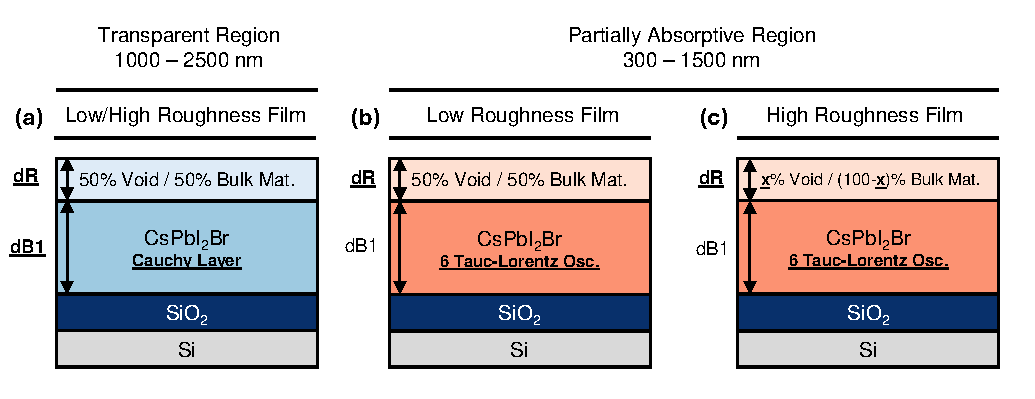
\includegraphics[width=.95\textwidth]{chapters/ellipsometry/image/Model_Approach.pdf}
  \caption{}
  \label{fig:ellipsometry:static_models}
\end{figure}

SE data are typically collected across a wide range of wavelengths (300 nm - 2500 nm) and at various angles of incidence (between 45\degree and 85\degree). This relatively simple dataset contains ample information about the physical material properties of a thin film (including its thickness, roughness, dielectric functions, uniformity, composition, and more), however a careful model-based regression analysis is required to extrapolate them. This means that a model of the sample has to be created, which of consists of fixed and fitted parameters. Fixed parameters are the known samples properties (e.g. the dielectric function of the substrate), while fitted parameters are all the unknown properties that are under investigation. An initial "guessing" of these unknown properties is necessary, followed by an iterative data-fitting process that compares the simulated and experimental $\Psi$ and $\Delta$ values. In the end, the quality of the fitting process is described by the mean squared error (MSE), given by: 




\begin{equation}
\text{MSE} = \frac{1}{N - M} \sum_{i=1}^{N} \left[ \left( \frac{\Psi_{\text{meas},i} - \Psi_{\text{model},i}}{\sigma_{\Psi,i}} \right)^2 + \left( \frac{\Delta_{\text{meas},i} - \Delta_{\text{model},i}}{\sigma_{\Delta,i}} \right)^2 \right]
\label{eq:mse}
\end{equation}

where \( N \) is the number of data points, and \( M \) is the number of fitting parameters. The quantities \( \sigma_{\Psi,i} \) and \( \sigma_{\Delta,i} \) denote the standard deviation of each experimental data point. Typically, achieving an MSE that is as low as possible is the objective. In the framework of this study, an MSE below 20 is considered necessary to ensure a good match between experimental and simulated values. 


For the characterization of perovskite thin films via spectroscopic ellipsometry, the following protocol can be followed for a foolproof model development: 
\begin{itemize}
    \item The spectral range is limited to a region where the perovskite film is transparent, i.e. below its bandgap value. In the case of our thermally evaporated \ch{CsPbI2Br} thin films (\ch{E_g} = 645 nm), we limit the spectral range between 1000 and 2500 nm. 
    \item In this region, the extinction coefficient (k) of the material is equal to 0, so the response of the material can be solely described by its refractive index (n), via the empirical Cauchy dispersion model:
        \begin{equation}
            n(\lambda) = A + \frac{B}{\lambda^2} + \frac{C}{\lambda^4}
            \label{eq:cauchy}
        \end{equation}
    \item Besides the A, B, and C values of equation \ref{eq:cauchy}, additional fitting parameters include the thickness of the perovskite bulk and the thickness of the roughness layer (as shown in Fig.~\ref{fig:ellipsometry:static_models}). The roughness is typically simulated as an additional layer, which follows the Bruggeman effective medium approximation (EMA), consisting of 50\% voids and 50\% bulk material, as introduced by Aspens et al \cite{Aspnes1979InvestigationEllipsometry}. 

    \item The relatively low number of fitting parameters, the interference of light reflected both from the sample's surface and the interface with the substrate, as well as the small influence of surface roughness in the infrared region render the Cauchy model ideal for a good estimation of the bulk thickness. 

    \item Having now bulk thickness as a fixed parameter, the Cauchy layer can be parameterized into a Kramers-Kroning consistent B-spline layer, extending the SE data range to the visible spectrum (up to 300 nm). 

    \item As a last step, the bulk's dielectric constant is further parameterized into a Generator Oscillator layer. (Low roughness film in Fig.\ref{fig:ellipsometry:static_fits}).    

\end{itemize}

Choosing the right type and number of oscillators in the last step is critical for the accurate determination of the film's optical constants. Using too few oscillators might make it impossible to reproduce the features in the experimental data, while using too many oscillators might lead to overfitting and the generation of results with little physical meaning. For the modeling of semiconductor materials, the use of Gaussian oscillator is the simplest choice. The imaginary part of the dielectric constant ($\varepsilon_r$) can be described by three free parameters, namely the amplitude ($A$), the broadening ($C$), and the center energy ($E_0$). However, the symmetric nature of the Gaussian oscillator does not fully describe the real optical transitions is thin films, where tail states and disorder lead to asymmetric broadening. As an alternative, Tauc-Lorentz oscillators are more commonly used for the modeling of perovskite thin films. This type of oscillator has one additional parameter that describes the bandgap energy of the material ($E_g$), producing a more asymmetric and realistic ($\varepsilon)2$) shape \cite{Jellison1996ParameterizationRegion}. Therefore, the absorption from the Tauc-Lorentz oscillator is described by: 

\begin{equation}
\varepsilon_2(E) =
\begin{cases}
\frac{A E_0 C}{E} \cdot \frac{(E - E_g)^2}{(E^2 - E_0^2)^2 + C^2 E^2}, & E > E_g \\
0, & E \leq E_g
\end{cases}
\label{eq:tauc_lorentz}
\end{equation}


The properties of perovskite thin films have been widely studied by means of SE measurements in literature. When measurements were performed in room temperature (RT), they were mainly used for the determination of the complex optical constants for various perovskite compositions \cite{Yan2020DeterminationFilms, Zhao2018EllipsometricFilm, Loper2015ComplexSpectrophotometry, Yuan2021Moisture-stimulatedProperties}. In a few occasions, SE in room temperature was used for less common studies, such as the identification of light-induced phase segregation \cite{Bernhardt2022InPerovskites} or the evaluation of perovskite degradation under ambient conditions \cite{Marronnier2018ElectricalConditions}. On the other hand, temperature-dependent SE measurements were previously performed on perovskite thin films for the characterization of their temperature-dependent optical properties \cite{Jiang2016TemperatureEllipsometry, Chen2019CharacterizingEllipsometry}, the investigation of temperature-induced degradation \cite{Tejada2022HybridInfrared, Wang2019InEllipsometry}, and the identification of phase-transition temperatures \cite{Yuan2020InPortfolio, Yuan2021Moisture-stimulatedProperties}. The following sections will identify specific limitations in the modeling of temperature-dependent SE data, will present a novel dynamic modeling approach, and will lastly provide new insights into the in situ annealing effect on thermally evaporated \ch{CsPbI2Br} thin films.  


\section{Temperature-Dependent SE for Perovskite Thin Films}

\begin{figure}[tbp]
  \centering
  \medskip
  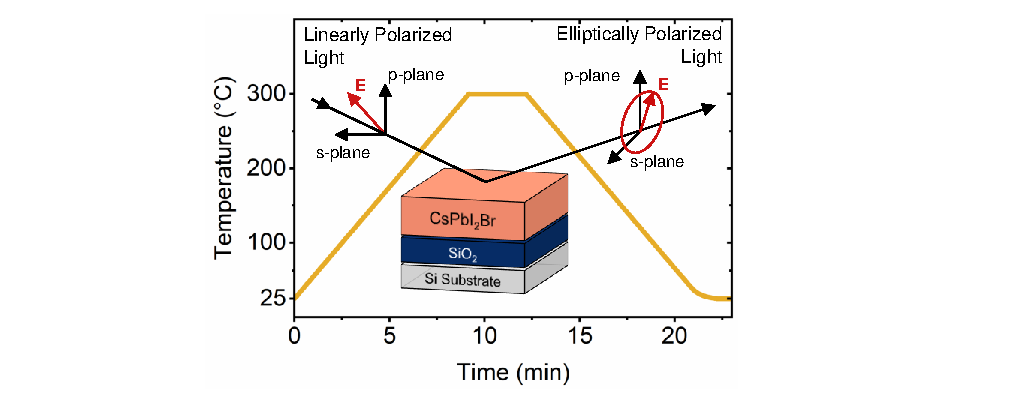
\includegraphics[width=.99\textwidth]{chapters/ellipsometry/image/experiment_description.pdf}
  \caption{}
  \label{fig:ellipsometry:experiment_description}
\end{figure}

\begin{figure}[htbp]
    \centering
    % First plot
    \begin{subfigure}[t]{0.95\textwidth} % Adjust width if needed
        \centering
        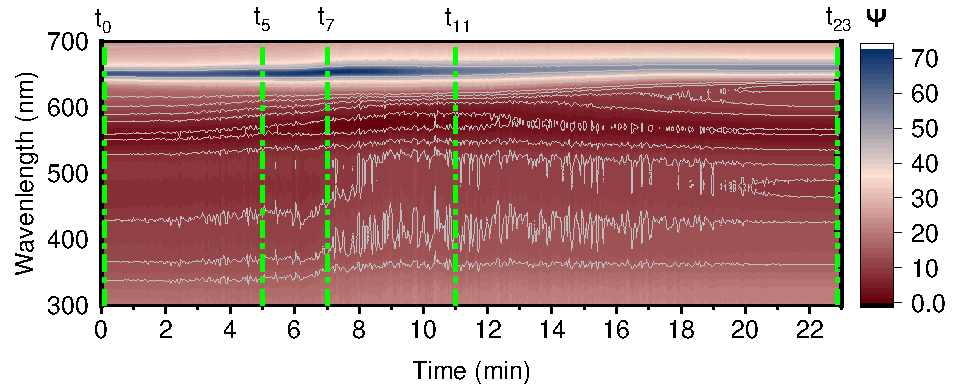
\includegraphics[width=\textwidth]{chapters/ellipsometry/image/Psi_Contour - MRS.pdf} % Replace with your image
        %\caption{Description for subplot (a).}
        %\label{fig:sub-a}
    \end{subfigure}

    \vspace{1em} % Space between the rows

    % Second plot
    \begin{subfigure}[t]{0.95\textwidth} % Adjust width if needed
        \centering
        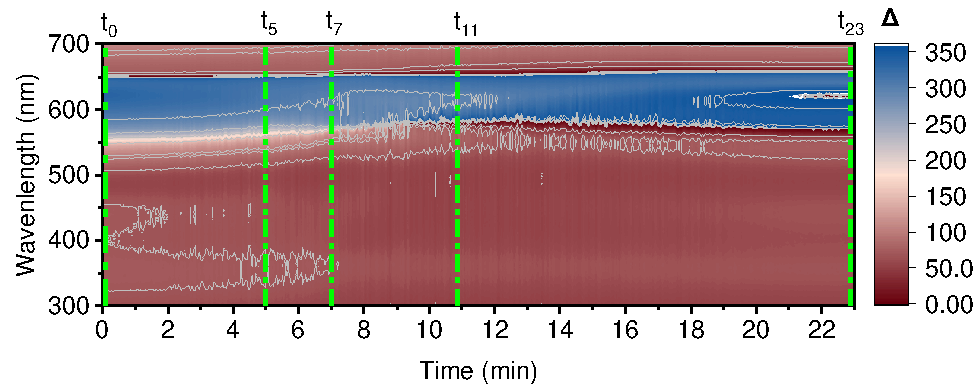
\includegraphics[width=\textwidth]{chapters/ellipsometry/image/Delta_Contour - MRS.pdf} % Replace with your image
        %\caption{Description for subplot (b).}
        %\label{fig:sub-b}
    \end{subfigure}

    % Caption for the whole figure
    \caption{}
    \label{fig:ellipsometry:raw_psi_delta}
\end{figure}

Most studies on temperature-dependent SE characterization follow an approach where they change the sample's temperature in step-wise increments or decrements, allowing for some stabilization time before moving to the next temperature step. A separate SE model is then developed for each temperature step. While this methodology ensures adequate time for potential transitions or internal structure changes, it is also likely that to conceal information around real-time effects. As an alternative, the implementation of a continuous heating ramp could be more representative of the changes that are taking place during a real annealing step. For this reason, we implemented the heating ramp shown in Fig.~\ref{fig:ellipsometry:experiment_description} for the characterization of an  \ch{CsPbI2Br} thin film, deposited on a Si substrate with 100 nm of thermally grown \ch{SiO_2}. This choice of substrate prevents complications arising from backside reflection in semitransparent substrates or multilayer interference within multilayer stacks. The sample was placed in a enclosed temperature stage that was continuously flushed with nitrogen. Starting from RT, the temperature was increased with a rate of approximately 30\degree C/min, up to 300\degree C. The sample was allowed to stabilize there for 3 minutes, before being cooled back down to RT with a rate of 35\degree C/min. An SE measurement at a fixed incident angle of 70\degree was taken approximately every 23 seconds. It would not be possible to perform varied angle SE due to the fixed position of the optical windows on the heating stage. The acquired $\Psi$ and $\Delta$ values
as function of time are shown in Fig.~\ref{fig:ellipsometry:raw_psi_delta}. Even though this data give some high level information about the moments the sample is going through drastic changes (e.g. between the $5^{\text{th}}$ and $11^{\text{th}}$ minute of the experiment), a careful modeling is necessary to decipher them. 

\begin{figure}
  \centering
  \medskip
  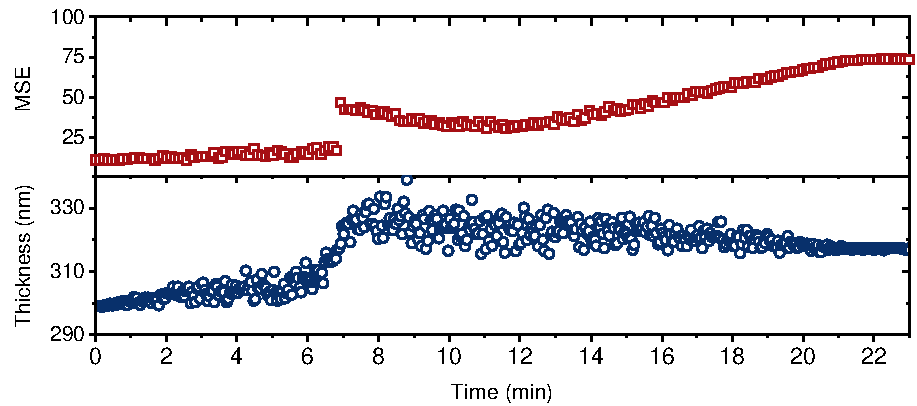
\includegraphics[width=.99\textwidth]{chapters/ellipsometry/image/wrong_model.pdf}
  \caption{}
  \label{fig:ellipsometry:wrong_model}
\end{figure}

However, the modeling of continuous SE data is not straightforward. One option that is facilitated by the software used for the analysis of the SE data (ComleteEASE) is the development of a static model for the initial state of the sample ($t_0$) (according to the protocol described in the previous section), followed by the dynamic fitting of its parameters as a function of time. We can expect that the thickness of the sample is changing due to thermal expansion, its roughness is increasing due to grain coalescence, and the position/energy of the oscillators are changing due to the energy that is transferred to the system. Therefore, for such a modeling approach 26 fitting parameters (1$\times$thickness, 1$\times$roughness, 6$\times$4 oscillators) should be turned-on. The continuous fitting of such a system is not only computationally heavy, it also entails the risk of overfitting. Some indicative results of such a modeling approach are demonstrated in Fig.~\ref{fig:ellipsometry:wrong_model}. Despite the fact that at the start of the experiment the MSE is reasonably low at the beginning of the measurement, it rises above 70 by the end of the experiment, pointing out to a large difference between measured and simulated data. Additionally, the predicted thickness of the film in the end of the measurement is almost 20 nm higher compared to the thickness of the as-deposited film. This is in contradiction with the profilometry results for the as-deposited and annealed state of the sample, which have approximately the same thickness, as shown in Fig.~\ref{fig:ellipsometry:profilometry}. Therefore, the continuous fitting of the initial static model is an unreliable way to model the acquired results. 


\begin{figure}
  \centering
  \medskip
  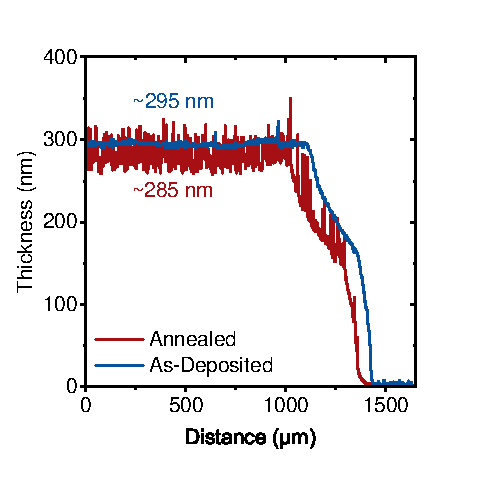
\includegraphics[width=.5\textwidth]{chapters/ellipsometry/image/Dektak.pdf}
  \caption{}
  \label{fig:ellipsometry:profilometry}
\end{figure}

An alternative modeling approach was inspired by a previous report on the modeling of aluminum gallium arsenide (\ch{Al_xGa_1_-_xAs}) optical constants as a function of composition \cite{Snyder1990ModelingComposition}. Specifically, considering that, for example, the optical constants of the compositions for $x=0.3$ and $x=0.4$ are known, then the optical constants of the intermediate composition for $x=0.35$ could be simulated through an EMA model of the two known compositions. Extending this concept to our experiment, we identified that it is possible to describe the complete temperature-dependent evolution of the perovskite thin film via a mixture of its optical constants at selected timestamps. This can be described by an EMA-based model, as shown in Fig.~\ref{fig:ellipsometry:dynamic_model}, where the bulk of the perovskite layer is a mixture of five static models, namely $sm1-t_0$, $sm-t_5$, $sm-t_7$, $sm-t_{\text{11}}$, and $sm-t_{\text{23}}$. The names of these static models represent the time frame they refer to, and they can be further distinguished in Fig.~\ref{fig:ellipsometry:raw_psi_delta}. The oscillator parameters of each static model are fixed. Only the volume fraction of each static model along with the bulk thickness and roughness thickness are set as fitting parameters. This creates a lightweight dynamic model with only 7 fitting parameters in total that can be fit in real time. The selection of these specific five static models was intentional: $sm1-t_0$ and $sm-t_{\text{23}}$ were included to account for the as-deposited and annealed state at RT, while $sm-t_{\text{11}}$ was included to account for the perovskite state at 300\degree C. Lastly, $\Psi$ and $\Delta$ values reveal that a major shift is happening to the composition of the perovskite around the $6^{\text{th}}$ minute of the experiment, motivating us to include two additional static models ($sm-t_5$ and $sm-t_7$) to account for the perovskite state before and after this shift. An essential condition for the accuracy of the dynamic EMA model is the accuracy of the constituents static models. For this reason, the following section provides a comprehensive analysis on the development of the static models, particularly for the as-deposited ($sm1-t_0$) and the annealed ($sm-t_{\text{23}}$) perovskite state, highlighting the impact of the surface roughness on the accuracy of simulated results. We specifically focus on the as-deposited and annealed state since the simulated results can be further corroborated through additional characterizations measurements before and after the annealing of the perovskite thin film. 

\begin{figure}
  \centering
  \medskip
  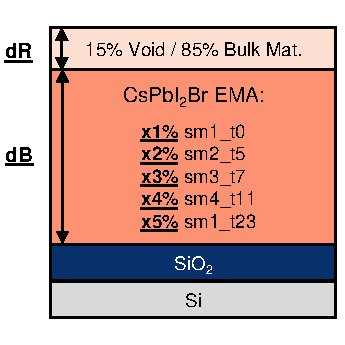
\includegraphics[width=.45\textwidth]{chapters/ellipsometry/image/Dynamic_Model.pdf}
  \caption{}
  \label{fig:ellipsometry:dynamic_model}
\end{figure}



\subsection{Static and Dynamic SE Model Development}

\begin{figure}[t]
    \centering
    % First row
    \begin{subfigure}[t]{0.45\textwidth}
        \centering
        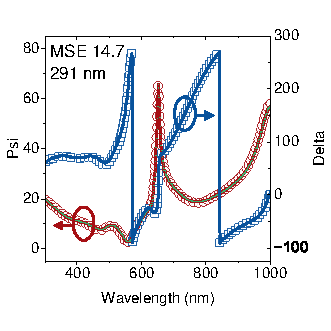
\includegraphics[width=\textwidth]{chapters/ellipsometry/image/t0_plot.pdf} % Replace with your image file
        \caption{As-Deposited State}
        \label{fig:ellipsometry:static_fits:t0}
    \end{subfigure}
    \hfill
    \begin{subfigure}[t]{0.45\textwidth}
        \centering
        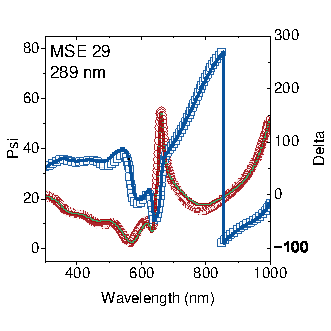
\includegraphics[width=\textwidth]{chapters/ellipsometry/image/t23_fixed_thickness_50_v.pdf} 
        % Replace with your image file
        \caption{Annealed State - Model A}
        \label{fig:ellipsometry:static_fits:t23_fixed_thick_50_void}
    \end{subfigure} 
 % Second row
    \begin{subfigure}[t]{0.45\textwidth}
        \centering
        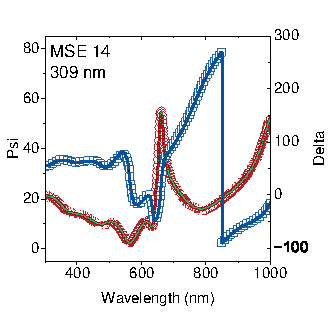
\includegraphics[width=\textwidth]{chapters/ellipsometry/image/t23_fitted_thickness.pdf} % Replace with your image file
        \caption{Annealed State - Model B}
        \label{fig:ellipsometry:static_fits:t23_fitted_thick}
    \end{subfigure}
    \hfill
    \begin{subfigure}[t]{0.45\textwidth}
        \centering
        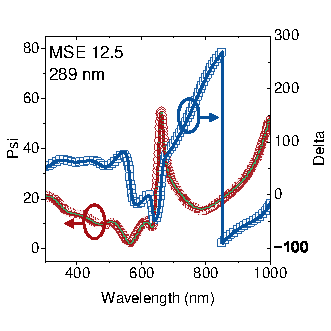
\includegraphics[width=\textwidth]{chapters/ellipsometry/image/t23_fixed_thick_x_void_p.pdf} % Replace with your image file
        \caption{Annealed State - Model C}
        \label{fig:ellipsometry:static_fits:t23_fixed_thick_x_void}
    \end{subfigure}
    \caption{}
    \label{fig:ellipsometry:static_fits}
\end{figure}

Developing a model for the as-deposited state ($sm1-t_0$) is rather straight forward, due to the relatively low surface roughness of the film (RMS = 2 nm, as seen in Fig.~\ref{fig:ch2:afm_before}). We consider that the interface between \ch{SiO_2} and \ch{CsPbI_2Br} is smooth with no intermixing between the layers. Following the protocol described in Section \ref{ch:ellipsometry:intro}, we extract a bulk thickness via a Cauchy model in the transparent region and get an approximation of 291 nm, which is consistent with the value provided by profilometry (295 nm in Fig.~\ref{fig:ellipsometry:profilometry}). The dielectric function of the film in the absorptive region is then modeled using 6 Tauc-Lorentz Oscillators, as shown in Fig.~\ref{fig:ellipsometry:static_models}, while the surface roughness is simulated through an additional EMA layer that consists of 50\% voids and 50\% bulk material. The fitting results of the $\Psi$ and $\Delta$ values are shown in Fig.~\ref{fig:ellipsometry:static_fits:t0}, where a good agreement between measurement and simulation is indicated via a relatively low MSE, equal to 14.7. To further corroborate the accuracy of the simulation, we extract the nk values for the as-deposited state and use them to simulate the film's absorptance and reflectance using the transfer matrix algorithm. Next, we experimentally evaluate the same parameters, via Reflectance/Transmittance measurements (R/T), considering the formula A(\%) = 100 - R(\%) - T(\%), where A stands for the film's absorptance. Fig.~\ref{fig:ellispometry:rt_as_dep} demonstrates a good agreement between experimental and simulated values, further corroborating the accuracy of the static model $sm1-t_0$.


\begin{figure}[htbp]
    \centering
    % First plot
    \begin{subfigure}[t]{0.49\textwidth} % Adjust width as needed
        \centering
        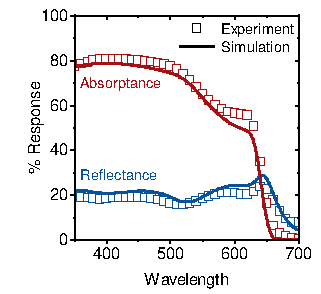
\includegraphics[width=\textwidth]{chapters/ellipsometry/image/RT_As_Deposited.pdf} % Replace with your image
        \caption{}
        \label{fig:ellispometry:rt_as_dep}
    \end{subfigure}
    \hfill % Space between the two plots
    % Second plot
    \begin{subfigure}[t]{0.49\textwidth} % Adjust width as needed
        \centering
        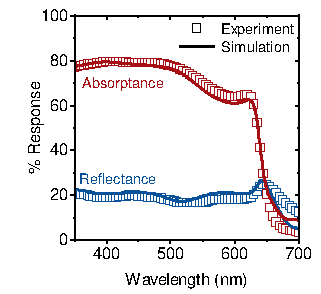
\includegraphics[width=\textwidth]{chapters/ellipsometry/image/RT_Annealed.pdf} % Replace with your image
        \caption{}
        \label{fig:ellipsometry:RT_annealed}
    \end{subfigure}

    % Caption for the whole figure
    \caption{Comparison of Absorptance and Reflectance}
    \label{fig:ellipsometry:RT}
\end{figure}

 
The development of a static model for the annealed perovskite state ($sm-t_{\text{23}}$) was not as straightforward. Using a Cauchy-based model in the transparent region, predicts the bulk thickness to be equal to 289 nm, which is consistent with the profilometry measurements of the annealed film (285 nm in Fig.~\ref{fig:ellipsometry:profilometry}). However, when trying to implement a model with 6-Tauc-Lorentz oscillators in the visible range, a larger discrepancy between experimental and simulated data is observed, as indicated through a higher MSE value (MSE = 29 in Fig.~\ref{fig:ellipsometry:static_fits:t23_fixed_thick_50_void}). It is possible to obtain a lower MSE by setting the bulk thickness as a fitting parameter (MSE = 14 in Fig.~\ref{fig:ellipsometry:static_fits:t23_fitted_thick}), however the newly estimated film thickness (309 nm) no longer matches with the experimental data. This challenge is attributed to the larger surface roughness of the annealed film (RMS = 28.5 nm in Fig.~\ref{fig:ch2:afm_after}). Specifically, the use of a 50:50 EMA layer for the modeling of the surface roughness is only a convention that should be used under the condition that the dimension of the roughness structure (D) is much smaller than the wavelength of the incident light ($\lambda$), expressed through the formula $D<0.1\lambda$. When D exceeds this limit, a complex EMA multilayer is typically necessary to describe the change in polarization due to increased light scattering \cite{Akagawa2011High-precisionEllipsometry}. It was shown that the surface roughness is commonly underestimated during the modeling of perovskite thin films via spectroscopic ellipsometry, leading to erroneous estimations of the films' optical constants \cite{Fujiwara2017DeterminationMaterials}. In the case of our thermally evaporated thin films, the shortest wavelength is $\lambda=300 nm$ and we can consider that D is equivalent to the RMS roughness measured with AFM ($D ~ 29$ nm), which is close to the boundary condition of $D<0.1\lambda$. This likely explains the challenge of developing a model that simultaneously achieves a realistic bulk thickness and a low MSE. 



However, considering that the boundary condition of $D<0.1\lambda$ is not exceeded, it is possible to overcome this modeling challenge without resorting to the use of complex multilayer structures. Instead, we demonstrate that it is possible to appropriately simulate the surface roughness by setting the percentage of voids in the roughness EMA layer as a fitting parameter, along with the layer's thickness. At the same time, the bulk thickness can be maintained as a fixed parameter, as illustrated in Fig.~\ref{fig:ellipsometry:static_models}. Indeed, using this approach, a lower MSE equal to 12.5 can be achieved (Fig.~\ref{fig:ellipsometry:static_fits:t23_fixed_thick_x_void}) for a roughness layer with approximately 15\% voids. To further corroborate the results of the simulation for the annealed state, we extract the nk values and use them to simulate the film's Absorptance and Reflectance, which prove to be in good agreement with the respective experimental values (Fig.~\ref{fig:ellipsometry:RT_annealed}). It has to be noted that neither experimental nor simulated data show a feature that could be attributed to the emergence of the 0D \ch{Cs_4PbI_4Br_2} phase that was revealed through the in situ GIWAXS measurements (Fig.~-giwaxs reference). This is in agreement with previous reports that investigated the emergence of the 0D \ch{Cs_4PbI_6} phase in 3D \ch{CsPbI_3} thin films \cite{Bai2019AStability}. Specifically, they showed that a discernible feature of the 0D phase only appears in the absorbance spectrum when the molar ratio between CsI and \ch{PbI_2} increases beyond 1.6:1.0. This ratio is much larger compared to the nominal ratio of CsBr:\ch{PbI_2} of 1.05:1.0 that was used for the deposition of our thin films. 

Having established the accuracy of the static models for the as-deposited and annealed state, we proceed with the development of the models for the three intermediate states, namely $sm-t_5$, $sm-t_7$, $sm-t_{\text{11}}$. Since the profile of roughness increase as a function of temperature is unknown, we fix the percentage of voids in the roughness layer to 15\% for all states. \textit{Table xx provides a summary of the information for all static models, including the MSE, the thickness of the bulk layer, the thickness of the roughness layer, as well as the percentage of voids.}


\begin{figure}[htbp]
  \centering
  \medskip
  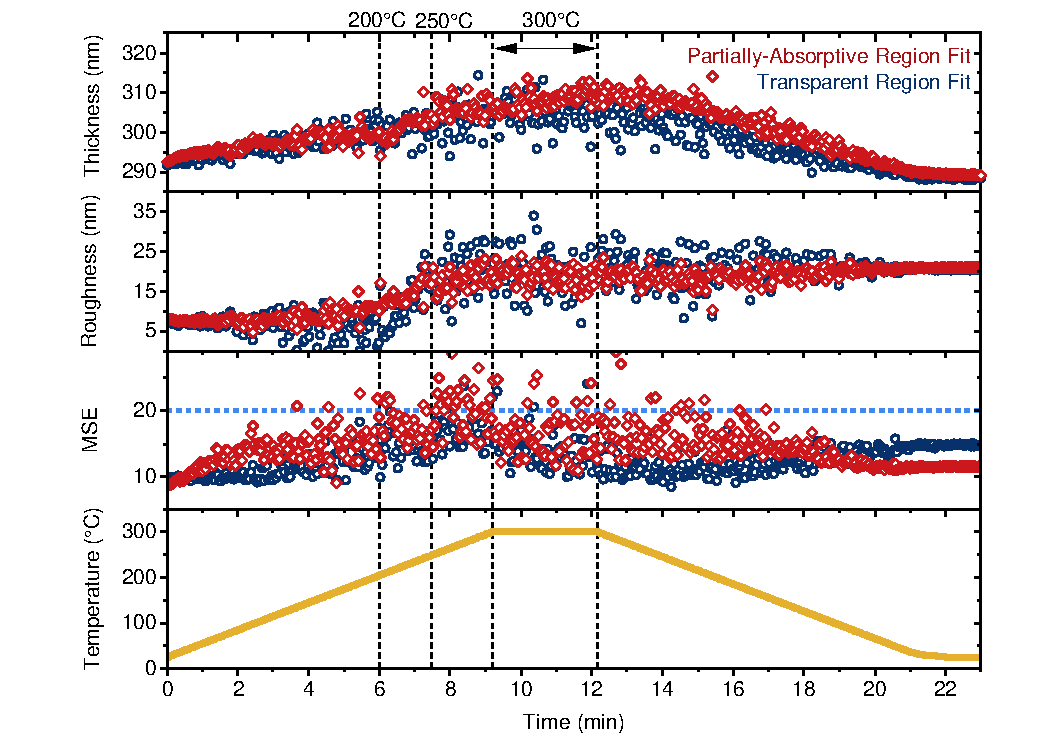
\includegraphics[width=.99\textwidth]{chapters/ellipsometry/image/Roughness_Thickness.pdf}
  \caption{}
  \label{fig:ellipsometry:roughness_thickness}
\end{figure}


As explained above, the changing properties of the perovskite thin film as a function of temperature can be described via an EMA model, which consists of 5 static models, mixed in different percentages. The dielectric functions of each static model are fixed, and only their volume ratio, along with the thickness of the bulk and roughness layers can vary. The percentage of voids in the roughness layer was again fixed at 15\%. Both the thickness and the optical constants of the \ch{SiO_2} layer are fixed, considering its particularly low thermal expansion coefficient ($0.5 \times 10^{-6} K^{-1}$), especially when compared to the thermal expansion coefficient of lead-iodide-based perovskites ($50\times10^{-6} K^{-1}$) \cite{Steele2019ThermalFilms}. Fig.~\ref{fig:ellipsometry:roughness_thickness} shows the evolution of MSE as a function of time and temperature, which is mostly maintained below 20 for the whole duration of the experiment. This provides a preliminary indication of the accuracy of the dynamic model, which will be further corroborated in the following sections through comparisons with literature and the results from additional characterization measurements. 

\section{In Situ Annealing Effect on Structural and Dielectric Properties}

Two types of scatter point are shown in Fig.~\ref{fig:ellipsometry:roughness_thickness}. The red scatter points represent the fitting results of the dynamic model (Fig.~\ref{fig:ellipsometry:dynamic_model}) in partially absorptive region (between 300 and 1000 nm). The blue scatter points represent the results of a simpler Cauchy-based model which is fitted in the transparent region (between 1000 and 2500 nm). The latter is not only more sensitive to thickness variations (due to light reflection from both the sample's surface and the sample-substrate interface),
but also simplifies the modeling of the roughness structure (the light wavelength is much larger compared to dimensions of the surface structure). As a result, the nearly identical trend in the evolution of the sample's thickness and roughness as a function of temperature that is observed between the two types of scatter points, can further strengthen the confidence in the results of our dynamic model. 


\begin{figure}[htbp]
  \centering
  \medskip
  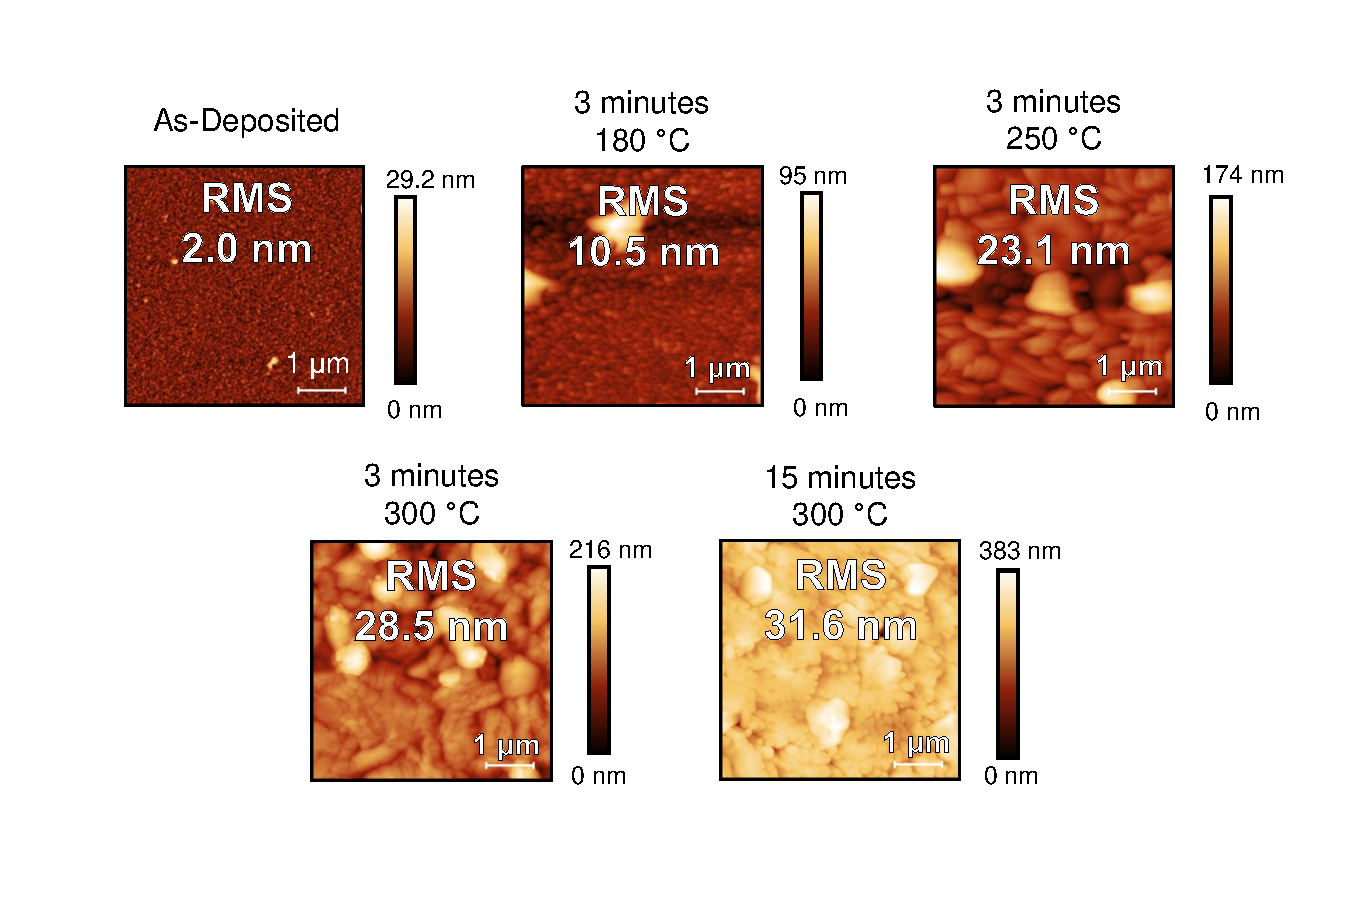
\includegraphics[width=1\textwidth]{chapters/ellipsometry/image/afm_all.pdf}
  \caption{}
  \label{fig:ellipsometry:afm_all}
\end{figure}


The results reveal that the sample's thickness is increasing linearly with temperature, despite the lattice phase changes that we know are happening. This is in agreement with what was observed by Marronnier et al, who used in situ synchrotron XRD measurements to report that the normalized unit cell volume of \ch{CsPbI_3} thin films varies linearly with temperature when transitioning sequentially from the the cubit to tetragonal and from tetragonal to orthorhombic phases \cite{Marronnier2018AnharmonicityCells}. Additionally, these results further agree with high thermal expansion coefficient that has been reported for lead halide perovskites, with our films exhibiting a thickness increase in the range of $1.7\times10^{-4}K^{-1}$. Of course, this value is depends a lot on the type of substrate, as an extension of the substrate-induced stress, but should anyways be taken into account when designing perovskite-based components that are meant to be exposed to high processing or operating temperatures. 

The perovskites roughness shows an intriguing and potentially counter-intuitive behavior. It has been generally shown for solution-processed perovskite thin films that the longer the annealing duration (and the higher the annealing temperature - not sure) the larger the size of grains eventually becomes. Even though it is not possible to extract direct information about the size of the film's grains through an SE measurement, it has been previously shown that the simulated thickness of the model's roughness layer has a linear relationship with the film's real roughness, measured through AFM measurements \cite{Fujiwara2000AssessmentFilms}. Hence, it is logical to associate the SE-derived roughness value with the size of the film's grains. It is observed that the film's roughness remains mostly stable (between 5 and 10 nm) until approximately 200 \degree C. At this point, a sharp increase is observed, before the roughness stabilizes again to a value close to 20 nm. To validate these results, we submit different thermally evaporated \ch{CsPbI_2Br} films to various annealing conditions. Fig. xx and xx shows the AFM scan for a film annealed for 3 minutes at 180 \degree C and 250 \degree C, respectively. Indeed, when the temperature is maintained below 200 \degree C, the average grain size remains below 150 nm, similarly to the morphology of the as-deposited state, while when the annealing temperature exceeds 200 \degree C, the average grain size increases to a range between 400 and 800 nm. The temperature threshold for the grain coalescence seems to coincide with the transition from the tetragonal to the cubic phase (190 \degree C, as revealed through in situ GIWAXS). It remains unclear whether grain coalescence is a direct consequence of the phase transition or if both mechanisms merely share a similar activation energy. Regardless, the increase in surface roughness observed in the SE data could serve as a signature for evaluating the tetragonal-to-cubic phase transition temperature in alternative thermally evaporated perovskite compositions. Further increasing the annealing temperature (300 \degree C) or extending the annealing duration (300 \degree C for 15 minutes) results in only a minor increase in the film's RMS roughness (from 28.5 to 31.6 nm), consistent with the plateau in roughness observed it the SE results. This analysis highlights that the grain size of thermally evaporated perovskite thin films depends more on the nucleation during the growth of the crystal, rather than the post-deposition annealing step. Therefore, future efforts for improved film quality via larger grains should be focused on the crystallization mechanism during the deposition rather than post-deposition treatments. 








\begin{figure}
  \centering
  \medskip
  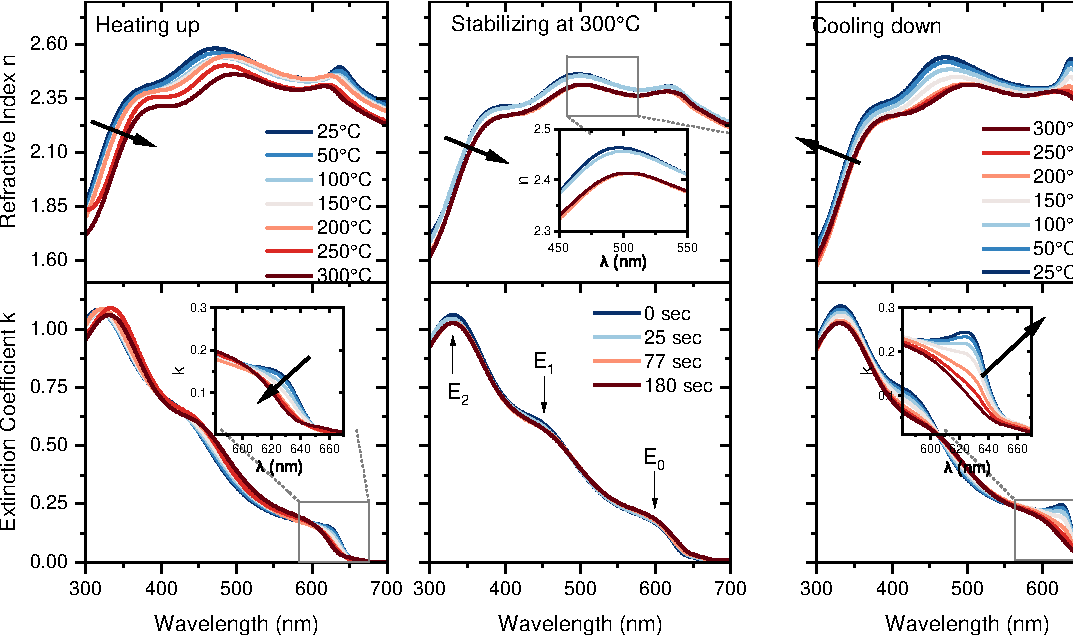
\includegraphics[width=.99\textwidth]{chapters/ellipsometry/image/Optical_constants.pdf}
  \caption{}
  \label{fig:ellipsometry:optical_constants}
\end{figure}


\subsection{Thermo-Optic Coefficient}

\begin{figure}[htbp]
    \centering
    \begin{subfigure}{0.32\textwidth}
        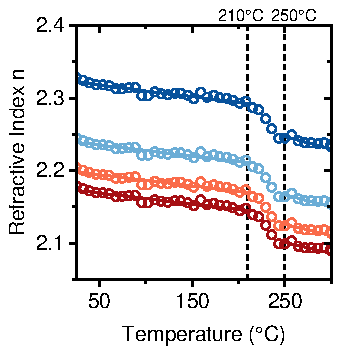
\includegraphics[width=\textwidth]{chapters/ellipsometry/image/Thermo-optic_Coefficient_heating.pdf}
        \caption{}
        \label{fig:ellipsometry:thermooptic_heating}
    \end{subfigure}
    \hfill
    \begin{subfigure}{0.32\textwidth}
        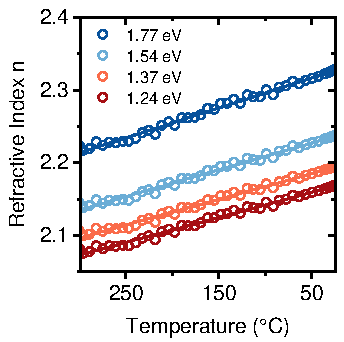
\includegraphics[width=\textwidth]{chapters/ellipsometry/image/Thermo-optic_Coefficient_cooling.pdf}
        \caption{}
        \label{fig:ellipsometry:thermooptic_cooling}
    \end{subfigure}
    \hfill
    \begin{subfigure}{0.3\textwidth}
        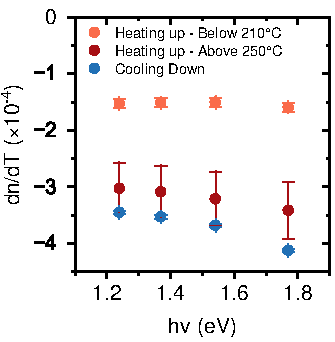
\includegraphics[width=\textwidth]{chapters/ellipsometry/image/Thermo-optic_Coefficient_energy.pdf}
        \caption{}
        \label{fig:ellipsometry:thermooptic_energy}
    \end{subfigure}
    \caption{A 1x3 figure layout.}
    \label{fig:ellipsometry:thermooptic}
\end{figure}



\subsection{Urbach Energy}

\begin{figure}[htbp]
    \centering
    \begin{subfigure}{0.32\textwidth}
        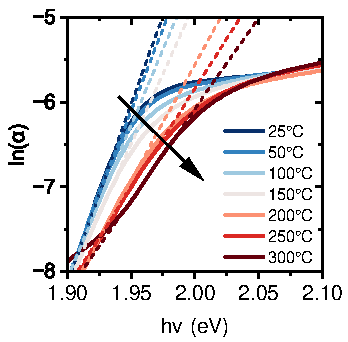
\includegraphics[width=\textwidth]{chapters/ellipsometry/image/Urbach_heating.pdf}
        \caption{}
        \label{fig:ellipsometry:urbach_heating}
    \end{subfigure}
    \hfill
    \begin{subfigure}{0.32\textwidth}
        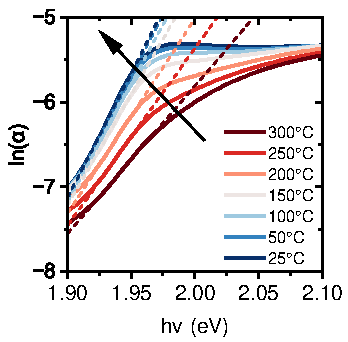
\includegraphics[width=\textwidth]{chapters/ellipsometry/image/Urbach_cooling.pdf}
        \caption{}
        \label{fig:ellipsometry:urbach_cooling}
    \end{subfigure}
    \hfill
    \begin{subfigure}{0.3\textwidth}
        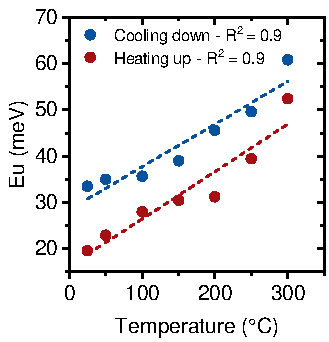
\includegraphics[width=\textwidth]{chapters/ellipsometry/image/Urbach_temp.pdf}
        \caption{}
        \label{fig:ellipsometry:urbach_temp}
    \end{subfigure}
    \caption{A 1x3 figure layout.}
    \label{fig:ellipsometry:urbach}
\end{figure}


\subsection{Critical Point Analysis}

\begin{figure}[htbp]
    \centering
    \begin{subfigure}{0.34\textwidth}
        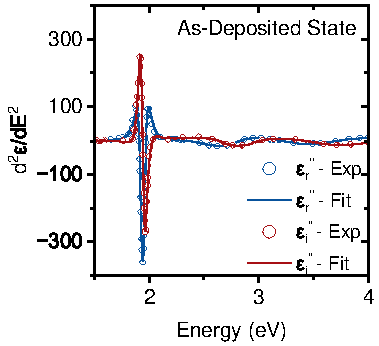
\includegraphics[width=\textwidth]{chapters/ellipsometry/image/Deriv_As_Dep.pdf}
        \caption{}
        \label{fig:ellipsometry:deriv:As_dep}
    \end{subfigure}
    \hfill
    \begin{subfigure}{0.31\textwidth}
        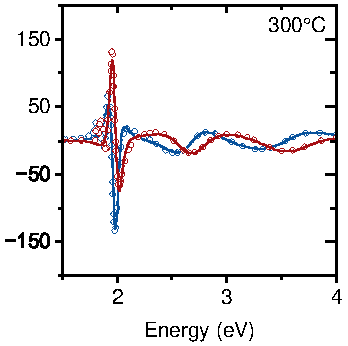
\includegraphics[width=\textwidth]{chapters/ellipsometry/image/Deriv_300C.pdf}
        \caption{}
        \label{fig:ellipsometry:deriv:300}
    \end{subfigure}
    \hfill
    \begin{subfigure}{0.31\textwidth}
        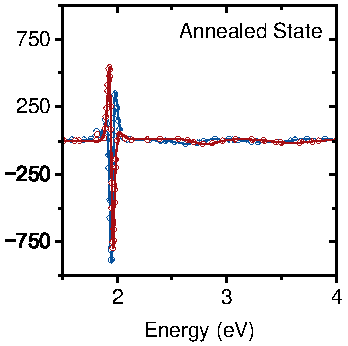
\includegraphics[width=\textwidth]{chapters/ellipsometry/image/Deriv_Anneal.pdf}
        \caption{}
        \label{fig:ellipsometry:deriv:anneal}
    \end{subfigure}
    \caption{A 1x3 figure layout.}
    \label{fig:ellipsometry:deriv}
\end{figure}

\begin{figure}[htbp]
    \centering
    \begin{subfigure}{0.34\textwidth}
        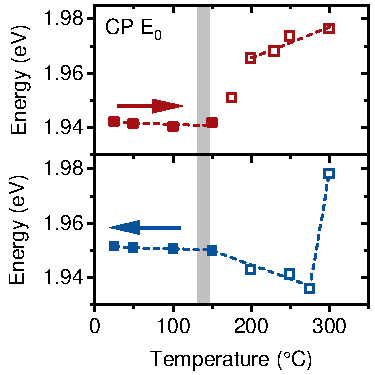
\includegraphics[width=\textwidth]{chapters/ellipsometry/image/CP0.pdf}
        \caption{}
        \label{fig:ellipsometry:CP0}
    \end{subfigure}
    \hfill
    \begin{subfigure}{0.31\textwidth}
        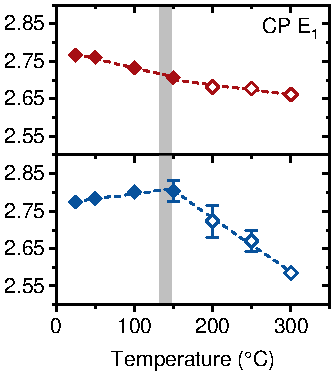
\includegraphics[width=\textwidth]{chapters/ellipsometry/image/CP1.pdf}
        \caption{}
        \label{fig:ellipsometry:CP1}
    \end{subfigure}
    \hfill
    \begin{subfigure}{0.31\textwidth}
        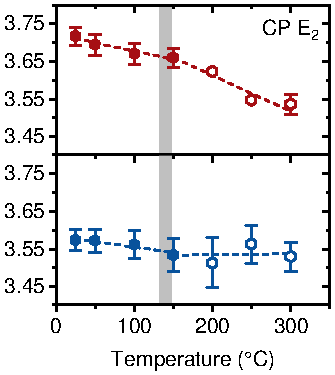
\includegraphics[width=\textwidth]{chapters/ellipsometry/image/CP3}
        \caption{}
        \label{fig:ellipsometry:deriv:CP2}
    \end{subfigure}
    \caption{A 1x3 figure layout.}
    \label{fig:ellipsometry:CP_all}
\end{figure}



\section{Conclusions}


%%%%%%%%%%%%%%%%%%%%%%%%%%%%%%%%%%%%%%%%%%%%%%%%%%
% Keep the following \cleardoublepage at the end of this file, 
% otherwise \includeonly includes empty pages.
\cleardoublepage

